% PGFPlots examples arranged as two text-width rows of subfigures.
\begin{subfigure}[t]{0.48\textwidth}
  \centering
  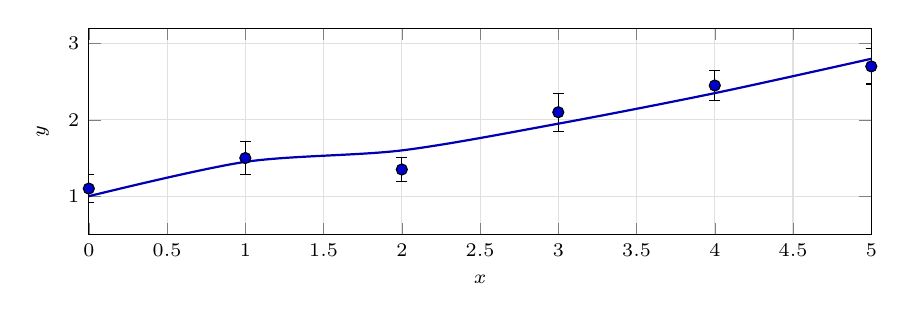
\begin{tikzpicture}
    \begin{axis}[
      width=.95\linewidth,height=42mm,
      tick label style={font=\scriptsize},label style={font=\scriptsize},
      grid=major,grid style={black!12},
      xlabel={$x$},ylabel={$y$},xmin=0,xmax=5,ymin=.5,ymax=3.2]
      \addplot+[only marks,black,mark=*,error bars/.cd,y dir=both,y explicit]
        coordinates {(0,1.1) +- (0,.18) (1,1.5) +- (0,.22) (2,1.35) +- (0,.16)
                     (3,2.1) +- (0,.25) (4,2.45) +- (0,.20) (5,2.7) +- (0,.23)};
      \addplot+[blue!70!black,no markers,thick,smooth]
        coordinates {(0,1.0) (1,1.45) (2,1.6) (3,1.95) (4,2.35) (5,2.8)};
    \end{axis}
  \end{tikzpicture}
  \caption{误差线曲线}
\end{subfigure}\hfill
\begin{subfigure}[t]{0.48\textwidth}
  \centering
  \begin{tikzpicture}
    \begin{axis}[
      width=.95\linewidth,height=42mm,
      tick label style={font=\scriptsize},label style={font=\scriptsize},
      grid=major,grid style={black!12},
      ylabel={频数},xmin=0,xmax=6,ymin=0,ymax=12,xtick={0,1,2,3,4,5,6}]
      \addplot+[ybar interval,fill=teal!28,draw=teal!70!black,line width=.5pt]
        coordinates {(0,1) (1,3) (2,8) (3,11) (4,7) (5,3) (6,1)};
    \end{axis}
  \end{tikzpicture}
  \caption{频数直方图}
\end{subfigure}

\par\medskip

\begin{subfigure}[t]{0.48\textwidth}
  \centering
  \begin{tikzpicture}
    \begin{axis}[
      width=.95\linewidth,height=42mm,
      tick label style={font=\scriptsize},label style={font=\scriptsize},
      grid=major,grid style={black!12},
      xlabel={$h$},ylabel={误差},xmode=log,ymode=log,
      xmin=.08,xmax=1.1,ymin=.001,ymax=.5,log ticks with fixed point,
      xtick={1,.5,.25,.125},ytick={.1,.01,.001},
      xticklabel style={/pgf/number format/fixed,/pgf/number format/precision=3}]
      \addplot+[mark=*,blue!70!black,thick] coordinates
        {(1,.32) (.5,.081) (.25,.020) (.125,.0051)};
      \addplot+[black,dashed,no markers,domain=.1:1,samples=40] {0.32*x^2};
    \end{axis}
  \end{tikzpicture}
  \caption{网格收敛曲线}
\end{subfigure}\hfill
\begin{subfigure}[t]{0.48\textwidth}
  \centering
  \begin{tikzpicture}
    \begin{axis}[
      width=.95\linewidth,height=42mm,
      tick label style={font=\scriptsize},label style={font=\scriptsize},
      xlabel={实验组},ylabel={观测值},
      boxplot/draw direction=y,xtick={1,2,3},xticklabels={A,B,C},ymin=.5,ymax=3.4]
      \addplot+[boxplot prepared={lower whisker=.8,lower quartile=1.1,median=1.5,
        upper quartile=1.9,upper whisker=2.3},fill=blue!18] coordinates {};
      \addplot+[boxplot prepared={lower whisker=1.0,lower quartile=1.4,median=1.8,
        upper quartile=2.4,upper whisker=3.0},fill=teal!18] coordinates {};
      \addplot+[boxplot prepared={lower whisker=.7,lower quartile=1.2,median=1.6,
        upper quartile=2.1,upper whisker=2.6},fill=orange!22] coordinates {};
    \end{axis}
  \end{tikzpicture}
  \caption{重复实验分布}
\end{subfigure}
